\documentclass{beamer}

\usepackage[ngerman]{babel}

\title{Text Klassifizierung}
\subtitle{logistische Regression und Support Vector Machines}
\author{Lukas Hofmaier \texttt{lukas.hofmaier@hsr.ch}}
\date{November, 2013 \\ Datenbanken Seminar HS13}

\begin{document}
\maketitle
\begin{frame}
  \frametitle{Outline}
  \tableofcontents
\end{frame}

\section{Problem}
\label{sec:problem}

\begin{frame}
  \frametitle{Problem}
  \begin{itemize}
  \item Zuordnung von Dokumenten zu Dokumentklassen
  \item System soll Zuordnung automatisiert ausf"uhren.
  \item generalisiertes Problem: Objekte zu bekannten Klassen zusammenfassen.
    \item richtige Zuordnungen (Trainingsdaten) sind gegeben. Algorithmus generiert Klassifizierer (supervised learning)
  \end{itemize}

\end{frame}

\begin{frame}
  \frametitle{Anwendungsbeispiele}
\begin{itemize}
\item Encoding detecting
\item Sprache in Dokument erkennen
\item Spamdetection
\item Sentiment detection
\item Automatisch e-Mail sortieren
\item Dokument-Ranking in Queryresult
\end{itemize}



\end{frame}

\section{Aufgabenstellung}
\begin{frame}
  \frametitle{Ergebnis}
  Artikel mit Analyse und Beschreibung von Klassifizierungsmethoden
  \begin{itemize}
  \item Problem der Textklassifizierung
  \item logistische Regression
  \item Support Vector Machine
  \end{itemize}
\end{frame}

\section{Inhaltsverzeichnis}
\label{sec:toc}

\begin{frame}
  \frametitle{Inhaltsverzeichnis}
  \begin{itemize}
  \item Problem der Textklassifizierung
    \begin{itemize}
    \item Vector Space Model
    \item TF-IDF Weight
    \end{itemize}
  \item Maschinelles Lernen
  \item logistische Regression
    \begin{itemize}
    \item Kostenfunktion
    \item Gradientenabstieg
    \item mehrere Klassen
    \end{itemize}
  \item Regularisation
  \item Support Vector Machine
    \begin{itemize}
    \item Large Margin Classifier
    \item Lagrange Funktion
    \item Kernel-Trick
    \item Sequential minimal optimization
    \end{itemize}
  \end{itemize}
\end{frame}

\section{Vector Space Model}

\begin{frame}
  \frametitle{Vector Space Model}
  \begin{itemize}
  \item Die Repr"asentation von Dokumenten als Vektoren nennt sich Vector Space Model
  \item jedes Dokument wird als Vektor repr"asentiert
  \item die Elemente sind TF-IDF Werte
  \end{itemize}

\end{frame}

\begin{frame}
  \frametitle{TF-IDF}
  $tf-idf$ Wert wird wie folgt berechnet:
\[
tf-idf_{t,d} = tf_{t,d} \times idf_t
\]

\begin{description}
\item[$tf_{td}$] term frequency. Wie oft tritt ein Wort $t$ in einem Dokument $d$ auf. 
\item[$idf_t$] Inverse document frequency. Bestimmt die Seltenheit eines Wortes $t$ in allen $N$ Dokumenten.
\end{description}

\[
idf_t = log \frac{ N}{df_f}
\]

\end{frame}

\section{logistische Regression}
\label{sec:logisticRegression}

\begin{frame}[fragile]
  \frametitle{Logistische Regression}
  \begin{columns}
    \begin{column}{.5\textwidth}

      \begin{block}{Decision Boundary}
        \[
        \theta_0 + \theta_1 x_1 + \theta_2 x_2 = 0
        \]
        \begin{description}
        \item[$x$] Featurevektor
        \item[$\theta$] Decisionboundary Parameter
        \end{description}
       \end{block}

      \begin{block}{Regel}
        Wenn $\theta^T x \geq 0$ dann $y=1$

        Wenn $\theta^T x < 0$ dann $y=0$
      \end{block}

    \end{column}
    \begin{column}{.5\textwidth}
      \begin{figure}
        \centering
        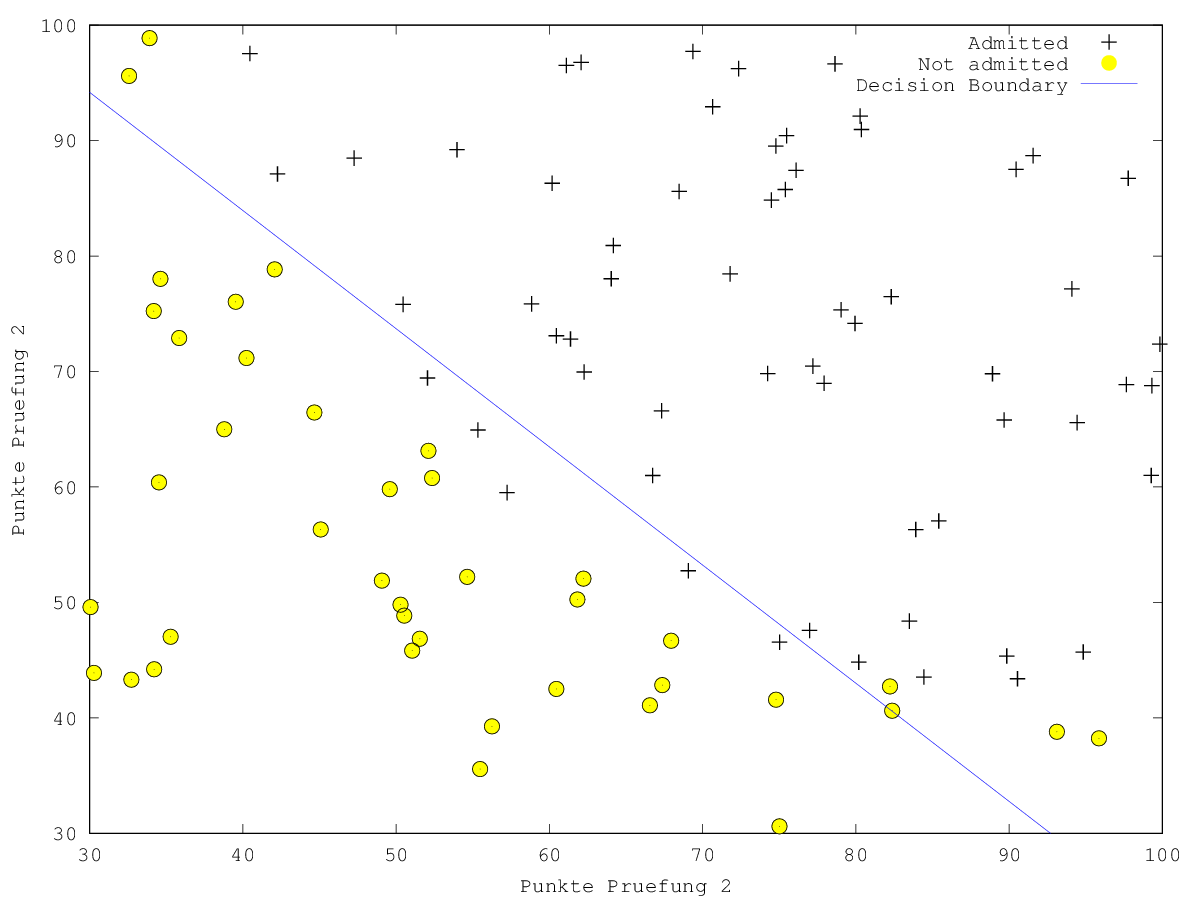
\includegraphics[scale=0.3]{decisionboundary}
      \end{figure}
    \end{column}
  \end{columns}
\end{frame}

\begin{frame}
  \frametitle{Kostenfunktion}

Die Funktion $h_{\theta}$ nimmt Punktezahl von Pr"ufung 1 und 2 und gibt einen Wert aus $0 \leq h_{\theta}(x) \leq 1$.

\[
J(\theta) = \left \{
\begin{array}{l l}
  -\log(h_{\theta} (x)) & \quad \text{if $y==1$}\\
  -\log(1-h_{\theta} (x)) & \quad \text{if $y==0$}
\end{array} \right.
\]

\[
J( \theta ) = - \frac{1}{m} \sum_{i=1}^m y^{(i)} \log h_{\theta}(x^{(i)}) + (1 - y^{(i)}) \log(1 - h_{\theta}(x^{(i)}))
\]
Der Funktionswert muss minimiert werden. Kann einfach mit Optimisierungverfahren minimiert werden (z.B. Gradientenabstieg)

\end{frame}

\section{Octave Demo}


\section{Ausblick}
\begin{frame}
  \frametitle{Ausblick}
  \begin{itemize}
  \item Zusammenfassen von erarbeitetem Wissen
    \begin{itemize}
    \item logistische Regression
    \item Regularisation
      \item SVM
    \end{itemize}
  \item Demonstration mit geeigneter Implementation von SVM vorbereiten
  \end{itemize}
\end{frame}
 

\begin{frame}
  \frametitle{weiterf"uhrende Literatur}

\begin{thebibliography}{Subramaniam, 2011}

\bibitem{manning}
Christopher D.Manning Prabhakar Raghavan Hinrich Sch"utze,
Introduction to Information Retrieval,
Cambridge
2008.

\end{thebibliography}
\end{frame}

\end{document}

